\documentclass{article}
%=================================================
% Basics
%=================================================
\usepackage{fixltx2e} % Makes \( \) equation style robust, among other
                      % things. Must be the first package.


% Makes ligatured fonts searchable and copyable in pdf readers
\usepackage{cmap} % Load before fontenc 

% Always include these font encodings in your document 
% unless you have a very good reason.
\usepackage[T1]{fontenc}
\usepackage[utf8]{inputenc}

\usepackage{verbatim}

%=============
% Fonts
%=============

\usepackage{lmodern} % Improved version of computer modern
\usepackage[scale=0.88]{tgheros} % Helvetica clone for sans serif font


\newcommand\hmmax{2} % Default is 3.
\newcommand\bmmax{2} % Default is 4.

\usepackage{bm} % boldmath must be called after the package
\providecommand{\mathbold}[1]{\bm{#1}}

%=============
% AMS Packages and fonts
%=============
\usepackage{amsmath,amsbsy,amsgen,amscd,amsthm,amsfonts,amssymb} 

%=============
% Margins and paper size
%=============
\usepackage[centering,top=1.5in,bottom=1.2in,left=1.4in,right=1.4in]{geometry}
\usepackage{parskip}


%=============
% Section headings
%=============
\usepackage[sf,bf,compact]{titlesec}

%=============
% Tables and lists
%=============
\usepackage{booktabs,longtable,tabu} % Nice tables
\setlength{\tabulinesep}{1mm}
\usepackage[font=small,margin=10pt,labelfont={sf,bf},labelsep={space}]{caption}

%=============
% Code output
%=============
% \usepackage{listings}
% \usepackage{minted}




\usepackage{enumitem}
\setitemize{itemsep=0pt} 
\setenumerate{itemsep=0pt}
\setlist{labelindent=\parindent,%  % Recommended by enumitem package
  font=\sffamily}


%=============
% Hyperlink colors
%=============
\usepackage[usenames,dvipsnames]{xcolor}
\definecolor{steelblue}{HTML}{A1BDC7}
\definecolor{orange}{HTML}{D98C21}
\definecolor{silver}{HTML}{B0ABA8}
\definecolor{rust}{HTML}{B8420F}
\definecolor{seagreen}{HTML}{2E6B69}
\definecolor{joshua}{HTML}{FBDC7F}
\definecolor{darksky}{HTML}{154c79}

\colorlet{steelblue}{silver!30!white}
\colorlet{darkorange}{orange!85!black}
\colorlet{darksilver}{silver!85!black}
\colorlet{darksteelblue}{steelblue!85!black}
\colorlet{darkrust}{rust!85!black}
\colorlet{darkseagreen}{seagreen!85!black}

\usepackage{url}
\usepackage[colorlinks=true]{hyperref}
\hypersetup{linkcolor=darkrust}    
\hypersetup{citecolor=darkseagreen}      
\hypersetup{urlcolor=darksilver}     

%=============
% Microtype
%=============
\usepackage[final]{microtype} 

%=====================
% Header
%=====================
% \usepackage{fancyhdr}
% \usepackage{nopageno} % Gets rid of page number at the bottom
% \fancyhf{} % Clear header style
% \renewcommand{\headrulewidth}{0.5pt} % remove the header rule
% \pagestyle{fancy}
% \fancyhead[LE,RO]{\textsf{\small \thepage}}
% 
% \setlength{\headheight}{14pt}
%=====================
% Fix delimiters
%=====================

% Fixes \left and \right spacing issues. See discussion at
% http://tex.stackexchange.com/questions/2607/spacing-around-left-and-right
\let\originalleft\left
\let\originalright\right
\renewcommand{\left}{\mathopen{}\mathclose\bgroup\originalleft}
\renewcommand{\right}{\aftergroup\egroup\originalright}

%=================================================
% Math macros
%=================================================

%=============
% Generalities
%=============
\usepackage{mathtools}
\mathtoolsset{centercolon}  % Makes := typeset correctly for definitions

%%% Equation numbering
%\numberwithin{equation}{section} 

%%% Annotations
\newcommand{\notate}[1]{\textcolor{red}{\textbf{[#1]}}}

%==============
% Symbols
%==============
\let\oldphi\phi
\let\oldeps\epsilon

\renewcommand{\phi}{\varphi}
\renewcommand{\epsilon}{\varepsilon}
\newcommand{\eps}{\varepsilon}

%==============
% Constants
%==============

% Set constants upright
\newcommand{\cnst}[1]{\mathrm{#1}}  
\newcommand{\econst}{\mathrm{e}}

\newcommand{\zerovct}{\vct{0}} % Zero vector
\newcommand{\Id}{\mathbf{I}} % Identity matrix
\newcommand{\onemtx}{\bm{1}}
\newcommand{\zeromtx}{\bm{0}}

%==============
% Sets
%==============
\providecommand{\mathbbm}{\mathbb} % In case we don't load bbm

% Reals, complex, naturals
\newcommand{\R}{\mathbbm{R}}
\newcommand{\C}{\mathbbm{C}}
\newcommand{\K}{\mathbbm{K}}
\newcommand{\N}{\mathbbm{N}}

%==============
% Probability
%==============
\newcommand{\Prob}{\operatorname{\mathbbm{P}}}
\newcommand{\Expect}{\operatorname{\mathbb{E}}}

%==============
% Vectors and matrices 
%==============
\newcommand{\vct}[1]{\mathbold{#1}}
\newcommand{\mtx}[1]{\mathbold{#1}}

\newcommand{\mrange}{\operatorname{range}}
\newcommand{\mnull}{\operatorname{null}}


\usepackage{graphicx}

\title{HW 2}
\author{Karl Hiner}
\date{\today}

\begin{document}
\maketitle	

\section{Boosting the perceptron}

\subsection{a}
Since the data are not linearly separable, we do not expect the algorithm to converge.
Describe how you choose your stopping criterion.

\textbf{Answer:}

Since convergence is not expected, and since we have a small number of training samples with which to do cross-validation,
I chose to simply stop at a fixed number of epochs.

I ran a simple search over an epoch count between 50 and 350, in increments of 25, and found that 50 epochs gave the best performance on the test set.
Setting the epochs to 50 gave a test accuracy of 96.49\%.
I will note, however, that even with one epoch, the perceptron acheived 92.11\% accuracy, and the accuracy values fluctuate rather than monotonicly increasing with the number of epochs.
This leads me to conclude that the perceptron does not truly learn much after the first pass through the data.
However, I still chose to use 50 epochs as the stopping criterion, since it gave the best performance, and it is still fast to execute.

Here is the code I used to run the search:

\begin{small}
\begin{verbatim}
# Search for the number of epochs that gives the best accuracy over the test set.
def find_best_epochs(X_train, y_train, X_test, y_test, min = 50, max = 350, step = 25):
    best_accuracy = 0
    best_epoch = 0

    for epochs in range(min, max + 1, step):
        perceptron = Perceptron(epochs=epochs)
        perceptron.fit(X_train, y_train)
        y_pred = perceptron.predict(X_test)
        accuracy = np.mean(y_pred == y_test)

        if accuracy > best_accuracy:
            best_accuracy = accuracy
            best_epoch = epochs

        print(f"Epochs: {epochs}, Test Accuracy: {accuracy * 100:.2f}%")

    print(f"Best Epochs: {best_epoch}, Best Test Accuracy: {best_accuracy * 100:.2f}%")
    return best_epoch

\end{verbatim}
\end{small}

\subsection{b}
Check your accuracy against a standard implementation such as \verb|sklearn|’s Perceptron function.
In particular, check your implementation’s accuracy against the classification accuracy (0-1 loss) of \verb|sklearn|’s implementation on the same test data (from above).
Explain any hyperparameter choices you make in calling \verb|sklearn|’s Perceptron, and whether these cause a discrepancy in the accuracy. 

\textbf{Answer:}
After some experimentation, I found a configuration that produced the exact same predictions as \verb|sklearn|'s perceptron model, with any number of epochs:
\begin{small}
\begin{verbatim}
# Custom:
Perceptron(learning_rate=learning_rate, epochs=epochs)

# sklearn:
SklearnPerceptron(eta0=learning_rate, max_iter=epochs, tol=None, shuffle=False)
\end{verbatim}
\end{small}

Here, \verb|learning_rate| is used by my custom \verb|Perceptron| class to the update multiplier, and \verb|epochs| is the number of epochs run.
To get the same results as \verb|sklearn|'s perceptron, I had to set \verb|tol=None| and \verb|shuffle=False|, since my perceptron does not shuffle the data or do early stopping.

With this configuration, and with 50 epochs over the training data, both my custom perceptron and \verb|sklearn| acheive 96.49\% accuracy over the test set.

\subsection{c}
Consider the data $\mtx{X} = \left[\vct{x}_1, \cdots, \vct{x}_m\right]^T$, where $\vct{x}_i \sim \mathcal{D}$ are iid.
For this part alone, assume that, with probability 1, the data are linearly separable with margin $\rho$ and that $\|\vct{x}\| \leq R$.
Prove that the Perceptron converges in at most $(R/\rho)^2$ steps.

\textbf{Answer:}

\begin{enumerate}
    \item \textbf{Update improvements}: After each update (misclassification),
    \begin{align*}
    \langle \vct{w}_{t+1}, \vct{w}^* \rangle &= \langle \vct{w}_{t} + y_t \vct{x}_{t}, \vct{w}^* \rangle\\
    &= \langle \vct{w}_{t}, \vct{w}^* \rangle + y_t \langle \vct{x}_t, \vct{w}^* \rangle&\text{Inner product is distributive}\\
    &\geq \langle \vct{w}_{t}, \vct{w}^* \rangle + \rho&\mtx{X} \text{ linearly separable with margin } \rho 
    \end{align*}
    This implies that $\langle \vct{w}_{t+1}, \vct{w}^* \rangle \geq t \rho$.
    \item \textbf{Norm increase}: After each update, the squared norm of the weight vector increases by at most \(R^2\):
    $$\|\vct{w}_{t+1}\|^2 = \|\vct{w}_t\|^2 + 2y_t \langle \vct{w}_t, \vct{x}_t \rangle + \|\vct{x}_t\|^2 \leq \|\vct{w}_t\|^2 + R^2$$

    This implies that $\|\vct{w}_{t+1}\|^2 \leq t R^2$.
\end{enumerate}

Using the above inequalities:
\begin{align*}
\langle \vct{w}_{t+1}, \vct{w}^* \rangle &\leq \|\vct{w}_{t+1}\| \|\vct{w}^*\|&\text{Cauchy-Schwarz inequality}\\
t \rho &\leq \|\vct{w}_{t+1}\| \|\vct{w}^*\|&\text{Inequality 1 above}\\
t \rho &\leq \sqrt{t} R \|\vct{w}^*\|&\text{Inequality 2 above}\\
t \rho^2 &\leq R^2  \|\vct{w}^*\|^2&\text{Simplify}\\
t &\leq \frac{R^2}{\rho^2}&\text{WLOG, set}\|\vct{w}^*\| = 1
\end{align*}
Note that we can set the norm of the optimal weight vector to 1 without loss of generality because we can scale the weight vector and the margin by the same amount without changing the classification.
That is, if $\vct{w}^*$ is a vector achieving margin $\rho$, then for some $c \in \mathbb{R}$, $c\vct{w}^*$ will achieve margin $\rho/c$.
In particular, this will not affect the ratio $R/\rho$.

Thus, the Perceptron algorithm will converge in at most \( (R/\rho)^2 \) steps.

\subsection{d}
Now, we shall implement AdaBoost with your Perceptron code from part (b) as the
weak learner.

Give your reasoning for how you would now choose the size of the training dataset for the weak learner.
Recall that a weak learner should have an error $< 1/2 - \gamma$, with $\gamma > 0$.
Derive a bound for $\gamma$ in terms of the sample size such that the probability of the weak learner making an error of $1/2 - \gamma$ is $> 1 - \delta$, for some $\delta > 0$.
State any PAC learnability assumptions you make.

\textbf{Answer:}

We make two PAC assumptions:
\begin{enumerate}
    \item \textbf{Realizability:} The data distribution allows for a weak learner to achieve an error rate \(< 1/2 - \gamma\).
    \item \textbf{IID:} The data is independently and identically drawn from this distribution.
\end{enumerate}
Let \(Z_i\) be the indicator random variable with \(Z_i = 1\) if the \(i\)-th example is misclassified by the weak learner, and \(0\) otherwise.
Let $\hat{e} = \frac{1}{m} \sum\limits_{i=1}^{m} Z_i$ be the empirical error, and let \(e\) be the true error.

Hoeffding's inequality tells us that for any \(\epsilon > 0\),
$$P(|\hat{e} - e| > \epsilon) \leq 2 \exp\left(-2m{\epsilon}^2\right).$$
Our objective is to have a true error \(e < 1/2 - \gamma\). However, we only have control over the empirical error \(\hat{e}\). To link this desired true error with the empirical error, we can freely set \(\epsilon = \gamma\).
That is, we aim to ensure the empirical error \(\hat{e}\) is within \(\gamma\) of the desired \(e < 1/2 - \gamma\), with high probability. Specifically, we want the probability of this not happening to be less than \(\delta\):
\begin{align*}
    2 \exp\left(-2m{\gamma}^2\right) &\leq \delta\\
    -2m{\gamma}^2 &\leq \ln\left(\delta/2\right)\\
    \gamma^2 &\geq \frac{-\ln\left(\delta/2\right)}{2m}\\
    \gamma &\geq \sqrt{-\frac{\ln(\delta/2)}{2m}}
\end{align*}
which is the bound for \(\gamma\) in terms of the sample size \(m\) and the confidence parameter \(\delta\) that we are looking for.

\subsection{e}
\subsubsection*{e1}
Implement your AdaBoost algorithm. Plot the accuracy (training and test) as a function of number of iterations.

\textit{Plotted below. I cannot figure out why my test accuracy is better than my training accuracy, but it casts doubt on my implementation.
I'm curious to compare with other implementations or if one is released in the answer guide.}

\subsubsection*{e2}
Plot the confidence margin, $\min_{x \in S}\|h(x)\|$, of your predictions vs number of iterations.

\textit{Plotted below. I've made many changes to my algorithm, with different results, but the basic shape is consistent - the confidence margin drops down to a relatively consistent near-zero value.
I interpret this as AdaBoost finding weak learners that contribute to the accuracy until it reaches the limit of its capacity, at which point it is unable to find any more weak learners that contribute to the accuracy.}

\begin{figure}
    \centering
    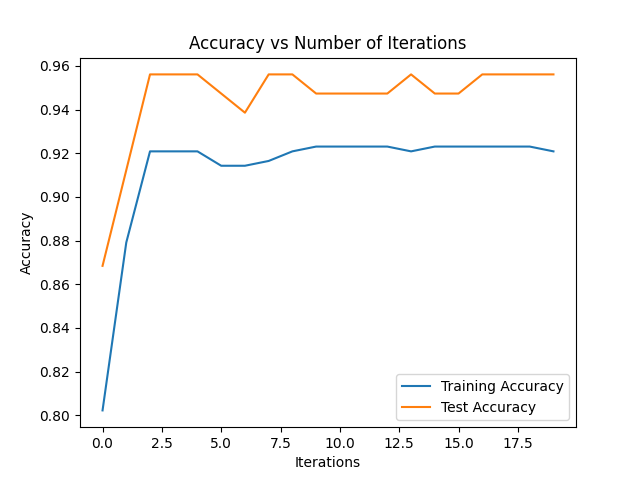
\includegraphics[width=0.8\textwidth]{images/adaboost_train_test_accuracy.png}
    \label{fig:boosting_accuracy}
\end{figure}

\begin{figure}
    \centering
    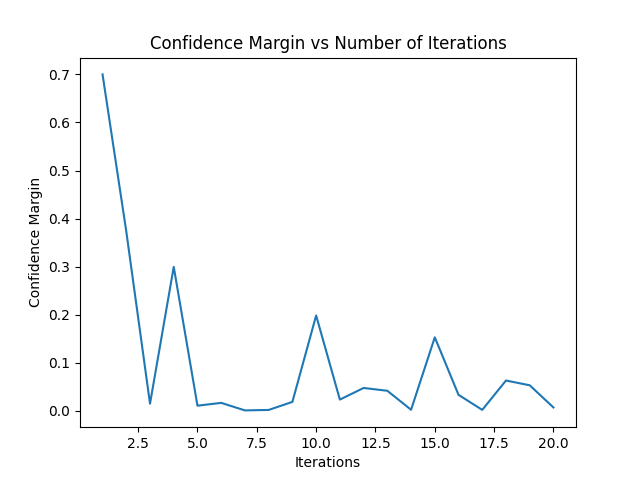
\includegraphics[width=0.8\textwidth]{images/adaboost_margin.png}
    \label{fig:boosting_margin}
\end{figure}
\clearpage

\subsection{f}

Let $f_t$ be your Perceptron output at iteration $t$ and $D_{t+1}$ be the updated distribution of the training points.
Generate iid samples from the $D_{t+1}$ in your code and plot the percentage of points misclassified by $f_t, f_{t - 1}$ at each $t$.
Analytically derive what this should be.

First, the analytical derivation.

In the textbook, in extension 10.3, we are given that
$$\frac{Z_{t+1}}{Z_t} \leq e^{-2\gamma^2},$$
where $Z_t = \frac{1}{m}\sum\limits_{i=1}^{m} e^{-y_i f_t(x_i)}$ is the normalization factor for the distribution $D_{t+1}$.

They further derive a tighter bound of $\frac{Z_{t+1}}{Z_t} \leq \sqrt{1 - 4\gamma^2}$.
Thus, we should expect to see in the plot a consistent relationship of $\frac{Z_{t+1}}{Z_t} \leq \sqrt{1 - 4\gamma^2}$.

My empirical results are plotted below.
\textit{Clearly, something is wonky about my implementation.
I've spent a lot of time trying different variations, introducing randomness to encourage diversity amongst weak learners, and modifying calculations for $D$ sample weights, among other things.
But I haven't been able to get the results to align with my interpretation of the theory.}

\begin{figure}
    \centering
    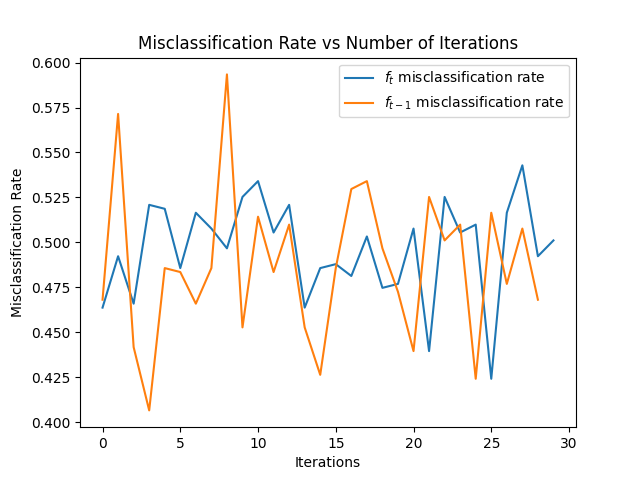
\includegraphics[width=0.8\textwidth]{images/adaboost_misclassification_rate.png}
    \label{fig:boosting_misclassification_rate}
\end{figure}

\clearpage

\subsection{g}
Describe your stopping criterion for AdaBoost.

\textbf{Answer:}

I simply use a fixed number of iterations as the stopping criterion for AdaBoost.

\subsection{h}
Explain your plots in part (e) using the results discussed in class about the effect of Boosting on the generalization error and margin.

\textbf{Answer:}
It seems clear that my empirical results at this time do not align with the theoretical expectations.
However, what we would \textit{expect} to see is that the training accuracy would increase consistently with the number of iterations, since AdaBoost focuses on the mistakes of the weak learners in previous iterations by re-weighting the training samples.
Thus, with each iteration, it's more likely to correctly classify previously misclassified samples.

In fact, in general AdaBoost should be able to achieve perfect accuracy by overfitting the training set.
Thus, we would expect to see the training accuracy approach 100\% as the number of iterations increases, while the test accuracy would reach a peak and then decrease as the model overfits the training data.

For the confidence margin, let's interpret what wthat e \textit{do} see in the results, which is a decreasing margin.
This suggests that AdaBoost is struggling to correctly classify challenging instances, and the ensemble's overall confidence in those instances is not improving despite adding more weak learners.

I interpret this as AdaBoost finding weak learners that contribute to the accuracy until it reaches the limit of its capacity, at which point it is unable to find any more weak learners that contribute to the accuracy.

\section{Support vectors}

Consider a classifier that returns the option 0 (reject) whenever $|yh(x)| \leq \rho$.
Recall the true risk/error, when considering the loss associated with a miclassification to be $1 : \Prob(Yh(X) < 0)$.

\subsection{a}
Let the class conditional density $\eta(x) = \Prob(Y = 1|X=x)$.
Suppose the loss value associated with returning the reject option, 0, is $c < 1/2$.
As with the 0-1 loss, the cost of misclassification, with confidence $yh(x) < -\rho$, is 1.
Derive an expression for the generalization error or Bayes risk, $R(h)$.

\textbf{Answer:}

The generalization error or Bayes risk, \( R(h) \), for a classifier \( h(x) \) can be formally defined as follows:
$$R(h) = \int \Prob(Y h(X) < 0 \mid X = x) p(x) dx$$
Here, \( \Prob(Y h(X) < 0 \mid X = x) \) is the probability of making an incorrect decision given that the feature vector \( X \) is \( x \). The integral runs over the entire input space, weighted by the data distribution \( p(x) \).

Let's decompose this term. An error happens in one of two scenarios:
\begin{enumerate}
    \item \( Y = 1 \) and \( h(x) < -\rho \), occurring with probability \( \eta(x) \)
    \item \( Y = 0 \) and \( h(x) > \rho \), occurring with probability \( 1 - \eta(x) \)
\end{enumerate}
Additionally, the classifier has an option to "reject", producing the output 0, with a cost \( c \) for both classes whenever \( |h(x)| \leq \rho \).

We will use the following shorthand labels for the three regions of the hypothesis space:
\begin{align*}
    A &\coloneqq \{ x : h(x) < -\rho \} \\
    B &\coloneqq \{ x : -\rho \leq h(x) \leq \rho \} \\
    C &\coloneqq \{ x : h(x) > \rho \}
\end{align*}
Now, we can express the total generalization risk as follows, where \( \mathbf{1}(\cdot) \) is the indicator function, which is 1 its argument is true and 0 otherwise:
\begin{align*}
    R_1 &\coloneqq \int \eta(x) \mathbf{1}(x \in A) p(x) dx\tag*{\text{\( Y=1 \) and \( x \in A \)}} \\
    R_0 &\coloneqq \int (1 - \eta(x)) \mathbf{1}(x \in C) p(x) dx\tag*{\text{\( Y=0 \) and \( x \in C \)}} \\
    R_c &\coloneqq c \int \left[ \eta(x) \mathbf{1}(x \in B) + (1 - \eta(x)) \mathbf{1}(x \in B) \right] p(x) dx\tag*{\text{\( Y=0 \) or \( Y=1 \) and \( x \in B \) } } \\
    &= c \int \left[ \eta(x) + (1 - \eta(x)) \right] \mathbf{1}(x \in B) p(x) dx\tag*{\text{Simplify} } \\
    &= c \int \mathbf{1}(x \in B) p(x) dx\tag*{\text{Final reject risk (independent of $\eta$)} } \\
    R(h) &= R_1 + R_0 + R_c\tag*{\text{Total generalization risk,}}
\end{align*}

\subsection{b}
The minimizer $h^*$ of the generalization risk is known to be of form
\begin{equation*}
h^*(x) = \begin{cases}
    -1 & \eta(x) < \delta\\
    0 & \delta \leq \eta(x) \leq 1 - \delta\\
    1 & \eta(x) > 1 - \delta
    \end{cases}
\end{equation*}
Show that $\delta = c$ minimizes the risk from part (a) with minimum risk being $E_X\min\{\eta(x), 1 - \eta(x), c\}$.

\textbf{Answer:}

To find the classifier \( h^* \) that minimizes the Bayes risk \( R(h) \), we will consider each term in \( R(h) \) individually. Recall from subsection (a) that \( R(h) = R_1 + R_0 + R_c \).

\begin{enumerate}
    \item The \( R_1 \) risk is minimized when \( \eta(x) < \delta \) and \( h(x) = -1 \).
    This is the lowest probability of misclassification for the positive class. 
    \item The \( R_0 \) risk is minimized when \( \eta(x) > 1 - \delta \) and \( h(x) = 1 \).
    This is the lowest probability of misclassification for the negative class.
    \item Finally, the \( R_c \) risk when choosing to "reject" will be \( c \).
    Since $c < 1/2$, this is lower than choosing either of the classes if \( \delta \leq \eta(x) \leq 1 - \delta \), with \( \delta = c \).
\end{enumerate}
Thus, the Bayes risk \( R(h^*) \) for the optimal classifier \( h^* \) can be found with:
\begin{align*}
    R(h^*) &= \min_{h} \left( R_1 + R_0 + R_c \right) \\
    &= \min_{h} \left[ \int \eta(x) \mathbf{1}(x \in A) p(x) dx + \int (1 - \eta(x)) \mathbf{1}(x \in C) p(x) dx + c \int \mathbf{1}(x \in B) p(x) dx \right] \\
    &= \int \min \left\{ \eta(x) \mathbf{1}(x \in A), (1 - \eta(x)) \mathbf{1}(x \in C), c \mathbf{1}(x \in B) \right\} p(x) dx \\
    &= \int \min \left\{ \eta(x), 1 - \eta(x), c \right\} p(x) dx \\
    &= E_X[\min \{ \eta(x), 1 - \eta(x), c \}] \quad \text{QED}
\end{align*}
That is, when the probability $\eta(x)$ is within a range where the risk of committing to a decision is higher than the fixed cost $c$, the optimal classifier prefers to reject.
This essentially enforces the notion that if the cost of making a \textit{wrong decision} is higher than the cost of \textit{not making a decision}, it is better to abstain.

\subsection{c}
Bartlett and Wegkamp 2008 define the following loss:
\begin{equation*}
l(z,h) = \begin{cases}
    1 - \frac{(1-c)yh(x)}{c} & yh(x) < 0\\
    1 - yh(x) & 0 \leq yh(x) \leq 1\\
    0 & yh(x) > 1
    \end{cases}
\end{equation*}
Note that the above loss is greater than the discontinuous loss in part (a).
When $c < 1/2 \leq \rho \leq 1 - c$, they show that the excess risk with this loss for any $h$ upper bounds the excess risk with the loss in part (a).
Write down an optimization problem for the ERM of this $l(z,h)$ loss using bounded, affine functions, i.e., $h_{w,b}(x) = w^Tx + b, \|w\| \leq r$.
Show that this optimization is convex.

\textbf{Answer:}

The ERM optimization problem is formulated as:
\begin{align*}
    \min_{w, b, \|w\| \leq r} \frac{1}{N} \sum_{i=1}^{N} l(y_i, h_{w,b}(x_i)),
\end{align*}
where \( h_{w, b}(x) = w^T x + b \) and \( \| w \| \leq r \).

Substituting \( l(z, h) \), we get:
\begin{align*}
    \min_{w, b, \|w\| \leq r} \frac{1}{N} \sum_{i=1}^{N} \begin{cases}
        1 - \frac{(1 - c) y_i (w^T x_i + b)}{c} & y_i (w^T x_i + b) < 0 \\
        1 - y_i (w^T x_i + b) & 0 \leq y_i (w^T x_i + b) \leq 1 \\
        0 & y_i (w^T x_i + b) > 1
    \end{cases}
\end{align*}
We can restate this using the indicator function \( \mathbf{1}(\cdot) \):
\begin{align*}
    \min_{w, b} \; & \frac{1}{N} \sum_{i=1}^{N} \left[\mathbf{1}(y_i (w^T x_i + b) < 0) \left(1 - \frac{(1 - c) y_i (w^T x_i + b)}{c}\right) \right. \\
    &\left. + \mathbf{1}(0 \leq y_i (w^T x_i + b) \leq 1) (1 - y_i (w^T x_i + b))\right],
\end{align*}
subject to \( \| w \| \leq r \).

Note that we simply drop the $y_i (w^T x_i + b) > 1$ component, since the loss in that domain is always 0.

The function inside the sum is piecewise linear.

To determine if this piecewise linear function is convex, set $\alpha \coloneqq y_i (w^T x_i + b)$, and compare the two lines representing the first and second piece:
\begin{enumerate}
    \item $y_1 = 1 - \frac{(1 - c)\alpha}{c}$
    \item $y_2 = 1 - \alpha$
\end{enumerate}
Observe that the slope of $y_2$ will be less than the slope of $y_1$ exactly when $c < 1/2$, which is the setting we are considering.
Thus, the function is convex.

Note that each term (sample pair) inside the summation of piecewise convex functions is piecewise \textit{over the same intervals} of the $yh$ domain.
Thus, the sum is also piecewise linear.

Finally, the constraints \( \|w\| - r \leq 0\) are affine.
Therefore, the optimization problem is convex.

\subsection{d}
Derive the KKT conditions for the problem in part (c).

\textbf{Answer:}

The KKT conditions consist of:

1. Stationarity:
\[
\begin{aligned}
    \nabla_w L &= \frac{1}{N} \sum_{i=1}^{N} \left[ -\mathbf{1}(y_i (w^T x_i + b) < 0) \frac{(1-c)y_i x_i}{c} - \mathbf{1}(0 \leq y_i (w^T x_i + b) \leq 1) y_i x_i \right] + 2 \alpha w = 0, \\
    \nabla_b L &= \frac{1}{N} \sum_{i=1}^{N} \left[ -\mathbf{1}(y_i (w^T x_i + b) < 0) \frac{(1-c)y_i}{c} - \mathbf{1}(0 \leq y_i (w^T x_i + b) \leq 1) y_i \right] = 0,
\end{aligned}
\]

2. Primal Feasibility:
\[
\| w \|  - r \leq 0,
\]

3. Dual Feasibility:
\[
\alpha \geq 0,
\]

4. Complementary:
\[
\alpha (\| w \|^2 - r^2) = 0.
\]

\subsection{e}

We are asked not to submit code, but I chose to anyway, since it took a good deal of work, and since we only received instructions for how to adjust our loss based on $\rho$ a day before the due date.

I believe the proposed method could be straightforwardly adapted into the \verb|custom_loss\| function below to penalize the separate conditions based on the deviation of $\rho$.

The test loss, without adjustment of $\rho$, is 0.109, which is already better than the 0-1 perceptron loss.

\begin{small}
\begin{verbatim}
import cvxpy as cp
import numpy as np
from sklearn.datasets import load_breast_cancer
from sklearn.model_selection import train_test_split

data = load_breast_cancer()
X = 2 * data.data - 1
y = 2 * data.target - 1
X_train, X_test, y_train, y_test = train_test_split(X, y, test_size=0.2, random_state=42)

N, D = X_train.shape
c = 1 / 3
r = 1

w = cp.Variable(D)
b = cp.Variable()
t = cp.Variable(N)

# Set up the constraints
constraints = []
for i in range(N):
    score = y_train[i] * (X_train[i, :] @ w + b)
    constraints.append(t[i] >= 1 - ((1 - c) * score / c))
    constraints.append(t[i] >= 1 - score)
    constraints.append(t[i] >= 0)

constraints.append(cp.norm(w) <= r)

# Set up the objective
objective = cp.Minimize(cp.sum(t) / N)

# Formulate and solve the problem
problem = cp.Problem(objective, constraints)
problem.solve()

# Extract the optimal values
w_opt = w.value
b_opt = b.value

# print(f"Optimal w: {w_opt}")
# print(f"Optimal b: {b_opt}")

def custom_loss(y, scores, c):
    loss_values = np.zeros(scores.shape)
    # Condition: y * score < 0
    mask1 = y * scores < 0
    loss_values[mask1] = 1 - ((1 - c) * y[mask1] * scores[mask1]) / c
    # Condition: 0 <= y * score <= 1
    mask2 = (y * scores >= 0) & (y * scores <= 1)
    loss_values[mask2] = 1 - y[mask2] * scores[mask2]
    # Condition: y * score > 1
    loss_values[y * scores > 1] = 0
    
    return np.mean(loss_values)

scores_test = X_test @ w_opt + b_opt
test_loss = custom_loss(y_test, scores_test, c)

print(f"Test loss: {test_loss}")
\end{verbatim}
\end{small}

\end{document}
